\documentclass[10pt]{article}
\usepackage[margin=0.65in]{geometry}
\usepackage{graphicx,parskip,hyperref}
\begin{document}
\begin{center}\Large Run0: retained failure and censored diagnostics\\
\normalsize 18 October2026; public ECC2K-130/F4 continuation\end{center}
\textbf{No GPU benchmark or frontier solve executed.} The archived packet
omitted two manifest-bound documents and the frontier script's executable
mode. All39 ECC source hashes passed, but the launch gate failed before
ECC execution. Hardware/ECC/negation/frontier exits were1/3/0/3. Root
retains this failed attempt and corrected delivery is a separate run.

The recovered archive has15,160 bytes and SHA256\\
\texttt{26d26efe1f6e8d9917c3256720065315dd37ee3c31ce909131139207938af217}.
Its file manifest and raw outputs are preserved under\texttt{remote/run-0/}.
Native hardware receipts identify RTX5090, driver580.65.06 and CUDA13.0;
these do not prove compatibility with the pinned CUDA13.3 build. The
instance exposes an AMD EPYC7663 and a124,999,999,488-byte memory cgroup.
No host-isolated timing claim is made.

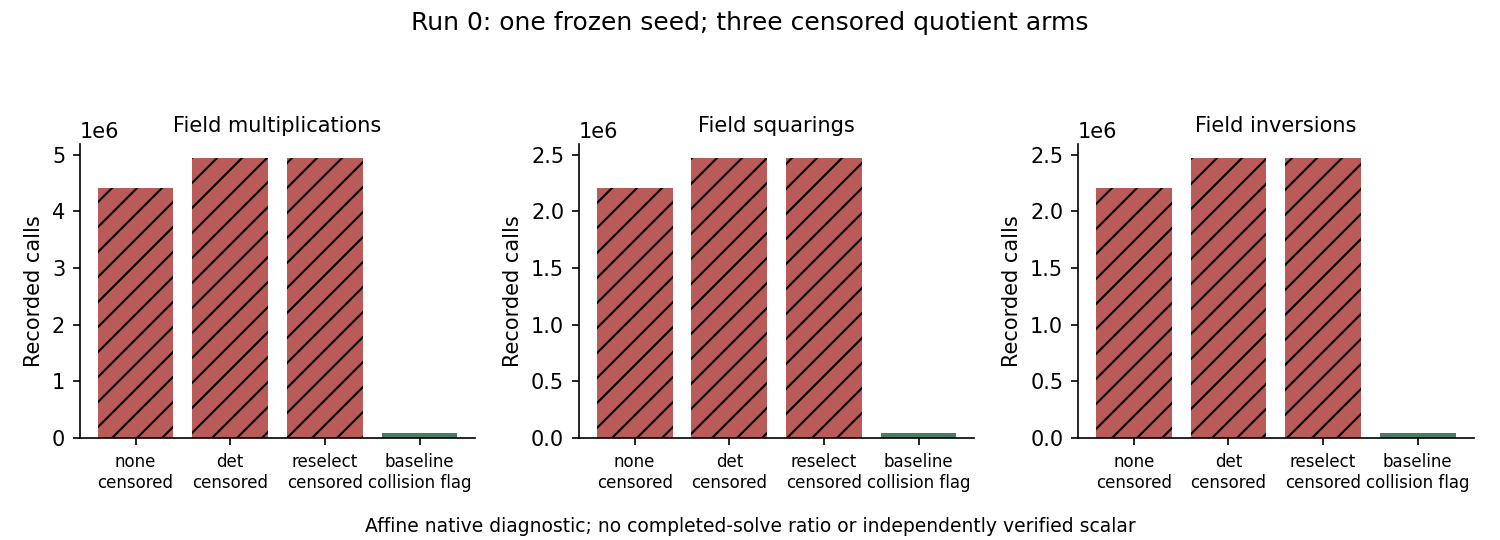
\includegraphics[width=\linewidth]{run0-operation-counters.png}

\textbf{All four commands returned0; three scientific outcomes are
censored.} The none/deterministic-break/reselect quotient arms each reached
2,208,379 steps without a collision. They reported0/1/1 distinguished
points. The baseline reported a collision after42,678 steps and10DPs.
The plotted multiplication/squaring/inversion counts are copied directly
from native outputs, with no M-equivalent conversion. Censored attempts
cannot supply a completed-solve ratio; a collision flag is not independent
verification of a recovered discrete logarithm.

The exact contract is H-RHO-bc6ea6 / EXP-RHO-60da4f. Its existing native
implementation uses affine arithmetic despite the specified Jacobian
model; that deviation and all existing censoring/control limits remain
explicit. This one-seed four-arm replay is instrument continuation only.

\textbf{Evidence.} See\texttt{RUN0\_RESULTS.md}, the native per-arm
\texttt{.command/.stdout/.stderr/.exit/.resources} files, launch source
verification, authenticated\texttt{http-job-status-run-0.json}, and the
original packet. A corrected run1 is separate and its outcome is not
asserted here. All original scientific acceptance criteria remain open
after run0. Canonical IC leaderboard and campaign rate figures are
unchanged: run0 adds no verified GPU throughput or complete ECDLP cost.
\end{document}
